\chapter{Single-Site Initial State with Interactions}\label{App:SingleSite_2p}

This appendix contains the results of simulations of two interacting particles, with $U=J$, initially on the same site. This gives a direct comparison to the single-particle simulations in Section \ref{Sec:SingleParticleResults}; however, since all Bloch bands are occupied, the behaviour is more complicated to analyse than the simulations which were instead presented in Section \ref{Sec:HexagonResults} with the hexagon initial state. 

Fig. \ref{Fig:Stationary_Density_2p} shows the density within $r=1.55\,a$ of the original site against time, as in Fig. \ref{Fig:Original_Site_Vicinity}. With $U\neq 0$, the particles do not remain localised indefinitely; instead, the density decays to $\sim0.1$ (approximately the value expected due to the average lattice filling). This qualitatively shows the effect of the interactions: the flat band degeneracy is lifted, and so the particles become mobile. 

The particle velocity in the flat band is significantly lower than in the dispersive bands, demonstrated by the timescales for the density in the original site vicinity to decay in Fig. \ref{Fig:Stationary_Density_2p} ($\sim$ 100s of $t_0$) and Fig. \ref{Fig:Original_Site_Vicinity} ($\sim 10\,t_0$). This is why simulations with this initial state are challenging to analyse more quantitatively. The dispersive density rapidly propagates around the lattice and interferes with the flat band density which is still slowly propagating away from the initial site, making it difficult to reliably extract parameters such as the decay time of the flat band density.

\begin{figure}[ht]
    \centering
    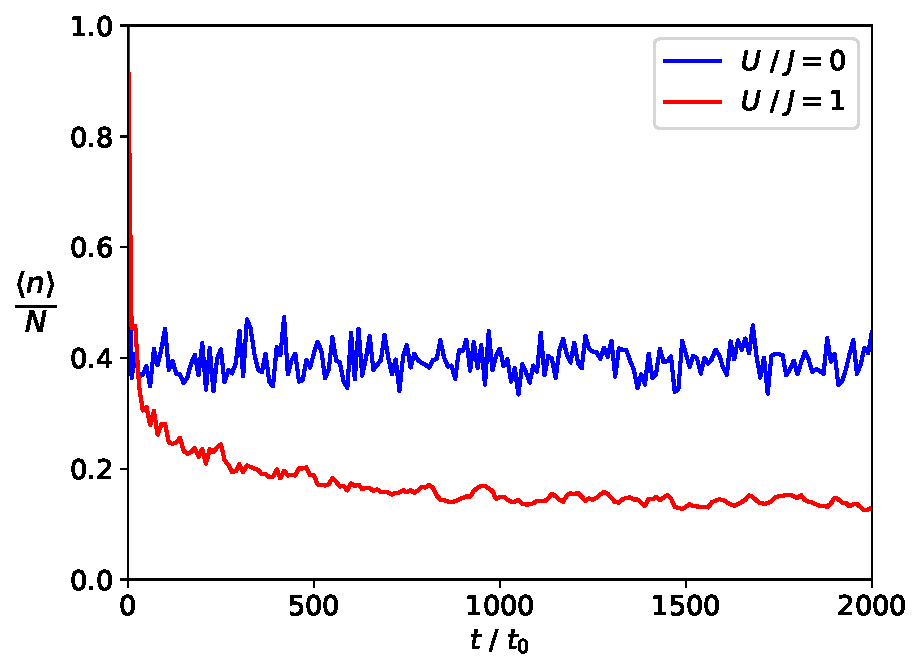
\includegraphics[width=10cm]{Figures/Stationary_Density_2p}
    \caption{Simulations of two particles initially on the same site, for interacting and non-interacting cases. Density within $r=1.55\,a$ of the initial site is plotted against time, as in Fig. \ref{Fig:Original_Site_Vicinity}. The density is normalized by the number of particles, $N=2$, to facilitate comparison to Fig. \ref{Fig:Original_Site_Vicinity}. The average lattice filling is higher for this 10$\times$10 unit cell lattice than for the 20$\times$20 lattice simulated in Section \ref{Sec:Staionary_Density_1p}, hence the density with $U/J=0$ remains significantly above 1/3. Open boundary conditions were used for these simulations, as in Section \ref{Sec:Staionary_Density_1p}.}
    \label{Fig:Stationary_Density_2p}
\end{figure}